\begin{activity}\label{A:0.3.1}
    Consider the function displayed in Figure \ref{F:0.3.Act1}.
    \ba
        \item Plot $-f(x)$ and $f(x)-1$.
        \item Define the function $g(x) = -f(x)-1$.  Does it matter which order you
            complete the tranformations from part (a) to result in $g(x)$?  Plot the
            functions resulting from doing the two transformation in part (a) in opposite
            orders.  Which of these functions is $g(x)$?
    \ea
    \begin{figure}[h!]
        \begin{center}
            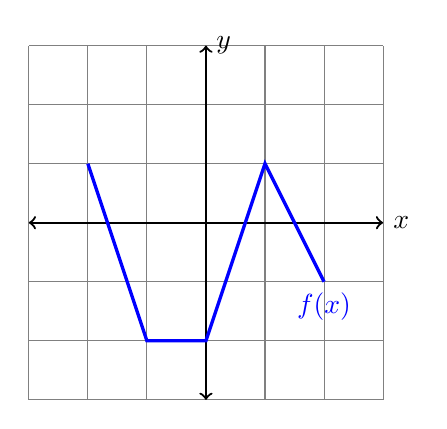
\begin{tikzpicture}[scale=0.75]
                \draw[color=gray] (-3,-3) grid (3,3);
                \draw[thick, black, <->] (-3,0) -- (3,0) node[anchor=west]{$x$};
                \draw[thick, black, <->] (0,-3) -- (0,3) node[anchor=west]{$y$};
                \draw[very thick, blue] (-2,1) -- (-1,-2) -- (0,-2) -- (1,1) -- (2,-1)
                node[anchor=north]{$f(x)$}; 
            \end{tikzpicture}
            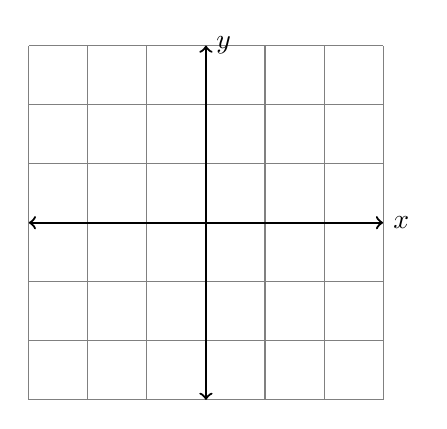
\begin{tikzpicture}[scale=0.75]
                \draw[color=gray] (-3,-3) grid (3,3);
                \draw[thick, black, <->] (-3,0) -- (3,0) node[anchor=west]{$x$};
                \draw[thick, black, <->] (0,-3) -- (0,3) node[anchor=west]{$y$};
            \end{tikzpicture}
        \end{center}
        \caption{Function transformation for Activity \ref{A:0.3.1}} \label{F:0.3.Act1}
    \end{figure}
\end{activity}\aftera
